%!TEX root = report.tex
\section{Methods \label{chapter2}}
%\subsection{Noise Design}
Some carefully designed \textsc{nmf} are robust to various noises. These robust algorithms aim to significantly reduce the amount of noise while preserving the edges without blurring the images \citep{barbu2013variational}. %Figure~\ref{noises} shows three kinds of noises we designed, including Gaussian noise, Poisson noise, and Salt \& Pepper noise.

\subsection{NMF and Gaussian noise}
\textbf{Gaussian noise} is noise with a probability density function being normal with mean zero. \citet{lee2001algorithms} propose the first \textsc{nmf} with the objective function between image~$V$ and its \textsc{nmf} factorisation~$W$ and~$H$ being
\begin{equation}
  \left\Vert V-WH \right\Vert= \sum_{ij} \left[V_{ij}-(WH)_{ij}\right]^2.\label{eq:obnmf}
\end{equation}
To minimise this object function of least square, \citet{lee2001algorithms} prove the convergence of the multiplication update rule
\begin{equation}
H_{jk}\leftarrow H_{jk}\frac{(W^{T}V)_{jk}}{(W^{T}WH)_{jk}} \text{ and } W_{ij}\leftarrow W_{ij}\frac{(VH)_{ij}}{(WHH^{T})_{ij}}.\label{eq:nmf}
\end{equation}
Here, $()_{ij}/()_{ij}$ denotes an entry-wise division of the two matrices. \citet{liu2015performance} show this \textsc{nmf} algorithm minimises Gaussian.

\subsection{KLNMF and Poisson noise}
\textbf{Poisson noise} or shot noise is a type of electronic noise that
occurs when the finite number of particles that carry energy,
such as electrons in an electronic circuit or photons in an optical
device, is small enough to give rise to detectable statistical
fluctuations in a measurement.
\citet{lee2001algorithms} suggest that \textsc{klnmf} is an algorithm that minimising the Kullback-Leibler divergence
\begin{eqnarray}
  D(V||WH)&=&\sum_{ij}\left(V_{ij}\log\frac{V_{ij}}{\left(WH\right)_{ij}}-V_{ij}+\left(WH\right)_{ij}\right)\nonumber\\
          &=&\sum_{ij}\left(-V_{ij}\log\left(WH\right)_{ij}+\left(WH\right)_{ij}+C(V_{ij})\right).\label{eq:klobj}
\end{eqnarray}
where $C(V_{ij})=V_{ij}\log V_{ij}-V_{ij}$. $C(V_{ij})$ is a function of the observed image matrix~$V$ only.
\citet{lee2001algorithms} also suggest a multiplication update rule to find as the optimisation procedure of \textsc{klnmf}
\begin{equation}
H_{jk}\leftarrow H_{jk}\frac{\sum_{i}W_{ij}V_{ik}/(WH)_{jk}}{\sum_{i'}W_{i'j}} \text{ and } W_{ij}\leftarrow W_{ij}\frac{\sum_{k}H_{jk}V_{ik}/(WH)_{jk}}{\sum_{k'}H_{ik'}}. \label{eq:klnmf}
\end{equation}
As this original image matrix~$V$ is observed, minimising this Kullback-Leibler divergence~\eqref{eq:klobj} is equivalent to minimising
\begin{equation*}
  \sum_{ij}\left(-V_{ij}\log\left(WH\right)_{ij}+\left(WH\right)_{ij}+C(V_{ij})\right).
\end{equation*},
for arbitrary bounded function~$C(V_{ij})$. Taking exponential of the negative of this score function, the problem transforms to maximising the following likelihood function
\begin{equation*}
L(WH|V)=\prod_{ij}\left(\left(WH\right)_{ij}^{V_{ij}}e^{-\left(WH\right)_{ij}}+C(V_{ij})\right).
\end{equation*}
Choosing constant $C(V_{ij})$ to be $-\log V_{ij}!$ gives
\begin{equation*}
L(WH|V)=\prod_{ij}\left(\frac{\left(WH\right)_{ij}^{V_{ij}}e^{-\left(WH\right)_{ij}}}{V_{ij}!}\right).
\end{equation*}
Hence, the probability density function of each element of the original matrix~V is Poisson
\begin{equation*}
P(V_{ij})=\frac{\left(WH\right)_{ij}^{V_{ij}}e^{-\left(WH\right)_{ij}}}{V_{ij}!}
\end{equation*}
is a sufficient condition to yield this likelihood. Hence \textsc{klnmf} is most suitable for images with Poisson noise.

\subsection{Preprocess}
We did not preprocess the images because both of \textsc{nmf} and \textsc{klnmf} are scale sensitive, because both objective functions~\eqref{eq:obnmf} and~\eqref{eq:klobj} varies when original matrix~$V$ and result matrices~$W$ and~$H$ scale proportionally, i.e. for $\lambda$ real, $D(V||WH)\neq D(\lambda V||\lambda WH)$. To overcome this issue, we could have normalised the matrices~$W$ and~$H$ in each iteration \citep{scaless}, but it will result in an even slower computation.

\subsection{Gaussian and Poisson are asymptotic equivalent}
 We design a Gaussian noise and a Poisson noise with different magnitude.
 Poisson distribution with parameter~$\lambda$ (integer) is equivalent to the sum of $\lambda$ Poisson distributions with parameter~$1$ \citep[][p. 45]{Walck:1996cca}.
 Hence for $\lambda$ large, Central Limit Theorem implies that Poisson distribution with parameter~$\lambda$ is well approximated by $N(\lambda,\lambda)$.
 When applying Poisson noise to an image, we do not have degree of freedom to choose any parameter.
 The variance is the magnitude of the pixels. To compare the robustness of \textsc{klnmf} with \textsc{nmf} with different noise, we choose the variance of Gaussian noise to be the difference from the magnitude of the pixel, that is, $N(0,\operatorname{Var})\neq N(0,V)\approx \operatorname{Poi}(V)-V$.
 Figure~\ref{noise} visualises the similarity of Poisson distribution and Normal distribution with parameter~$V=40$. To overcome this issue, the Gaussian noise we use should have very different variance in comparison with the mean of the images. The pixel mean of the \texttt{ORL} dataset is approximately $40$, and the pixel mean of the Cropped Yale set is approximately $70$. Hence, we choose the variance of the noise to be $80^2$ so that it is the way bigger than $255$, which is the maximum value of a pixel.
\begin{figure}
  \centering
  % Requires \usepackage{graphicx}
  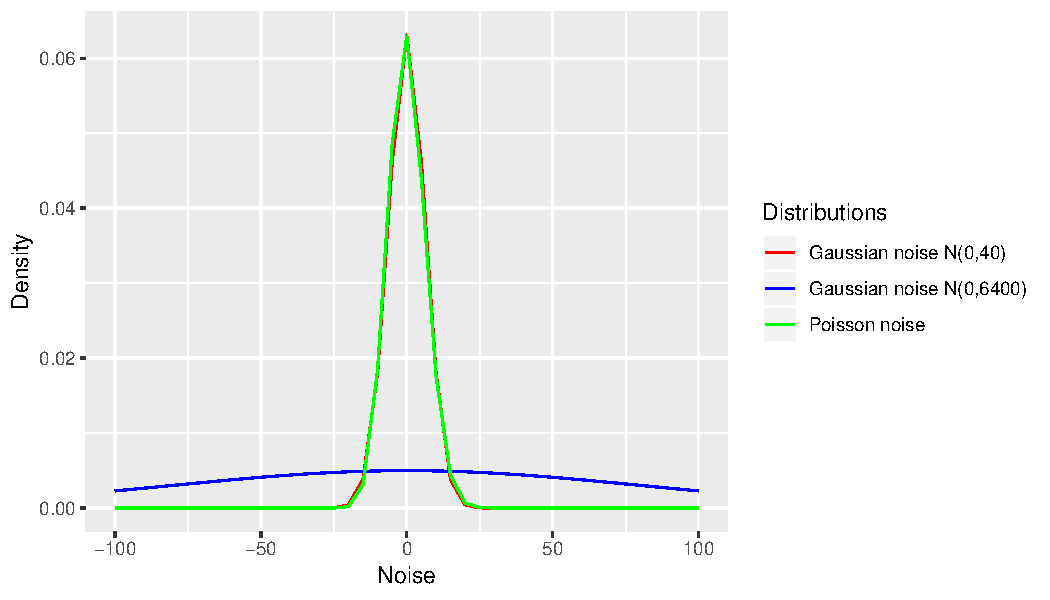
\includegraphics[scale=.8]{noise}\\
  \caption{Compare a Gaussian noise~$N(0,40)$ with Poisson noise $\operatorname{Poi}(40)-40$. They two distributions are asymptotically equivalent and have overlapped density functions. The Gaussian noise~$N(0,80^2)$ is very different.}\label{noise}
\end{figure}

\subsection{Salt \& Pepper noise}
Apart from Gaussian and Poisson noises, we also test our two algorithms on the commonly seen \textbf{Salt \& Pepper noise}. The noise presents itself by having dark pixels in bright regions and bright pixels in dark regions \citep{sampat2005computer}.

\subsection{Multiple initial estimates assure the algorithms stable}
As discussed in the section of related work,
The problem of nonnegative matrix factorization is not a convex problem.
Hence the results update rules~\eqref{eq:nmf} and~\eqref{eq:klnmf} coverage to maybe local minima instead of global minima, depending on the initial approximation.
Our task was to compare the robustness of the algorithm, and we do not want the instability of our algorithms to affect our comparison.
To address this issue, we implement several (i.e. $n$) initial estimates for each matrix factorisation problem.
We use the factorised matrices~$W$ and~$H$ corresponding to the least residual~\eqref{eq:obnmf} and~\eqref{eq:klobj}, for \textsc{nmf} and~\textsc{klnmf}, algorithms respectively, as the final result of factorisation.
This design of multiple starting point improves the stability of the algorithms, but it requires more computational power. To improve the computational speed, we make the number~$n$ equal to the number of cores of the \textsc{cpu}. We assign each of the $n$ initial estimates randomly with a uniform distribution. Then these each of the $n$ initial estimates is assigned to a different core of the \textsc{cpu}. This boosts the \textsc{cpu} utilisation to 100\% instantly and improved the computational speed by 70\% on the \texttt{ORL} data. The following part of our code implements this idea of parallel computing.
\begin{lstlisting}[caption=Multi-start paralle computing, label=matn1]
args = zip(repeat(V,ncpu), repeat(r,ncpu), repeat(niter[name2],ncpu), repeat(min_error[name2],ncpu))
result = pool.starmap(algo, args)
\end{lstlisting}
where \texttt{algo} is the \textsc{nmf} algorithm and \texttt{niter} is the number of iterations. We use a 16-thread Xeon high performance computer to run this algorithm.
 The algorithms run in this high performance computer so that the computing time is reasonable.  The multiple initial estimates assure the algorithms are stable.

% \begin{figure}\label{hpc}
%  \centering
%  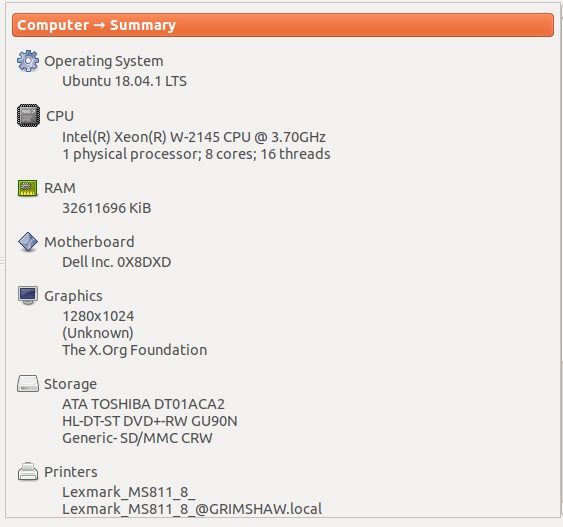
\includegraphics[scale=.5]{hpc}
%  \caption{}
%\end{figure}



\subsection{KLNMF requires more iterations}
A residual versus the number of iteration plot (figure~\ref{error}) shows that \textsc{klnmf} converges slower than \textsc{nmf}. In the log-log plot, the slope of the \textsc{nmf} residual plot is $2.5$ times larger than that of the \textsc{klnmf} plot for the \texttt{ORL} data. The slope estimates that the rate of convergence of \textsc{nmf} is $2.5$ faster than \textsc{klnmf}. As a result, we set the number of iterations as $500$ and $1200$ for \textsc{nmf} and \textsc{klnmf} algorithms, respectively (i.e. roughly $2.5$ more iterations).
 \begin{figure}
  \centering
  % Requires \usepackage{graphicx}
  \includegraphics[scale=.8]{error}\\
  \caption{Residual of the objective function~\eqref{eq:obnmf} and~\eqref{eq:klobj} versus the number of iterations. \textsc{nmf} converges more than twice faster than \textsc{klnmf}.}\label{error}
\end{figure}

\subsection{Evaluation metrics and their confidence intervals \label{ci}}
The assignment instruction asks us to compare the performance of \textsc{nmf} and \textsc{klnmf} by using evaluations metrics including Relative Reconstruction Errors (\textsc{rre}), Average Accuracy (\textsc{aa}), Normalized Mutual Information (\textsc{nmi}). The instruction states the formulae of these metrics. However, to systematically compare the metrics, we construct an 95\% confidence interval for any metric (e.g. \textsc{rre}) by bootstrapping percentile confidence interval. The idea of bootstrapping  is straightforward---we resample a subset of $40$ samples among the sample space of $80$ Monte-Carlo simulations and calculate the mean. We repeat this process $1000$ times. The $2.5\%$ and $97.5\%$ percentiles of the $80$ resampled means are then the bootstrapping percentile confidence interval
\begin{equation}
(\textsc{rre}^*_{2.5}, \textsc{rre}^*_{97.5}), \label{eq:boot}
\end{equation}
where $\textsc{rre}^*_{\alpha}$ is the $\alpha$ percentile of the bootstrapped distribution from our sample space with $80$ Monte-Carlo simulations.  We run $80$ simulations so that the confidence interval we construct is precise.

Bootstrapping does not require the sample space follows specific distributions. We apply this nonparametric method to construct confidence interval here because we do not know about the exact distributions of these three evaluation metrics.

\subsection{Statistical method compares the robustness of algorithms}
We implement the Kolmogorov-Smirnov test to test the hypothesis that the algorithms~\textsc{nmf} and~\textsc{klnmf} have different robustness. Again Kolmogorov-Smirnov test is distribution free, so we do not need to know the distributions of the evaluation metrics.

Let $\textsc{rre}_i$ denote the \textsc{rre} generated from our \textsc{nmf} algorithm by the $i$th Monte-Carlo simulation. Define the empirical distribution of a sample set generated by algorithm~$\alpha$, perhaps the $80$ \textsc{rre} results, as
\begin{equation}\label{epdf}
  \hat{F}_{\alpha}(x)=\frac{1}{n}\sum_{i=1}^{80}1_{\textsc{rre}_i \leq x}.
\end{equation}
The test statistic is the supremum among the differences of the empirical distribution generated using definition~\eqref{epdf} \citep{Walck:1996cca}
\begin{equation}\label{teststatistic}
D=\sup _{x}\left|F_{\alpha_2}(x)-F_{\alpha_2}(x)\right|.
\end{equation}
We compare the test statistics~$D$ with the critical value of $0.215$, which corresponds to $80$ samples and a 95\% of confidence level. We reject the null hypotheses that the two algorithms produce similar \textsc{rre} (or other evaluation metrics) with 95\% confidence level if the test statistics~$D>0.215$. The technique is extended to compare \textsc{aa} and \textsc{nmi}.
%\csvautobooktabular{{"../results/statistics".csv}}
%\subsection{Preprocessing}
%We apply global centring and local centring to preprocess the image data~\texttt{Vhat}
%\begin{lstlisting}[caption=Centring image data, label=matn1]
%n_samples = len(Vhat)
%# global centering
%Vhat = Vhat - Vhat.mean(axis=0)
%# local centering
%Vhat -= Vhat.mean(axis=1).reshape(n_samples, -1)
%Vhat -= Vhat.min()
%\end{lstlisting}
